\lstset{language=Java, numbers=left, numberstyle=\tiny, stepnumber=2, numbersep=5pt}
\chapter{Introduction}
\label{key}
In the last few decades software has become an important factor in everyone's lives. New and exciting developments in this sector can be observed every day by those who are interested. This ranges from simple applications used for smartphones which are basically used by all people around the globe to more abstract and complex things like self driving cars or automated houses. The goal is to make all people's lives more comfortable. Work that is too dangerous or too exhausting is done mostly by machines these days. Although this is a development which is greatly appreciated by most people, it brings some problems as well. As software is developed by people, it can never be fully reliable. People make mistakes and this transfers to the programs they write.\\
This leads to the question how a better reliability and stability can be achieved for our programs. The answer of course is \textbf{testing}.\\
There are a lot of different methods, guides, processes and tutorials on this topic. These cannot be all listed here in this document, because it would be too long. There are manual tests which can be done by the developer or the user himself by just using the software and later reporting bugs he found and other problems. But in most cases this happens too late, because the software is usually already delivered and deployed. This makes fixing bugs and changing the problematic code a lot more difficult.\\
It is easier to observe the stability and reliability of a software earlier during the development process by using automated tests such as unit-, regression- and integration-tests. One development process making good use of these automated tests is \textbf{Test Driven Development} or \textbf{TDD}. TDD will be further explained in the next chapter.

%%%%%%%%%%%%%%%%%%%%%%%%%%%%%%%%%%%%%%%%%%%%%%%%%%%%%%%%%%%%%%%%%%%%%%%%%%%%%%%%%%%%%%%%%%%%%%%%%%%%%%%%%
%%%%%%%%%%%%%%%%%%%%%%%%%%%%%%%%%%%%%%%%%%%%%%%%%%%%%%%%%%%%%%%%%%%%%%%%%%%%%%%%%%%%%%%%%%%%%%%%%%%%%%%%%
%%%%%%%%%%%%%%%%%%%%%%%%%%%%%%%%%%%%%%%%%%%%%%%%%%%%%%%%%%%%%%%%%%%%%%%%%%%%%%%%%%%%%%%%%%%%%%%%%%%%%%%%%
\chapter{Test Driven Development}
\label{tdd}
Test Driven Development (TDD) is a software development and design paradigm which centers very specific tests to be the indicator for the development process \cite[see][]{Bec04}. The test-cases which represent the requirements for the tested class are specified and integrated before the actual code that needs to be tested is implemented. Necessary specifications such as class- and method names are made at the beginning of the development cycle for a specific class. Every single test should fail at first, because the tested methods won't do the work they need to, because they aren't implemented yet. After that the actual code is implemented and will be further corrected and developed until it satisfies the requirements and all tests turn green, when they are run again.  \cite[see][]{WMV03}.\\
In TDD it is not allowed or recommended to integrate new functionality for software when the corresponding tests do not exist yet.\\
The goal of this approach is improving code quality and ensuring that the code fulfills the needed requirements while slowly teaching the developers to write better testable code.\\
Unit Tests can be developed for almost all existing programming languages. There are a lot of different frameworks such as NUnit\footnote{\url{http://www.nunit.org/}} for .NET developers or JUnit\footnote{\url{http://www.junit.org/}} for Java-users. In this assignment, JUnit will be used, because the code is written in Java.

%%%%%%%%%%%%%%%%%%%%%%%%%%%%%%%%%%%%%%%%%%%%%%%%%%%%%%%%%%%%%%%%%%%%%%%%%%%%%%%%%%%%%%%%%%%%%%%%%%%%%%%%%
%%%%%%%%%%%%%%%%%%%%%%%%%%%%%%%%%%%%%%%%%%%%%%%%%%%%%%%%%%%%%%%%%%%%%%%%%%%%%%%%%%%%%%%%%%%%%%%%%%%%%%%%%
%%%%%%%%%%%%%%%%%%%%%%%%%%%%%%%%%%%%%%%%%%%%%%%%%%%%%%%%%%%%%%%%%%%%%%%%%%%%%%%%%%%%%%%%%%%%%%%%%%%%%%%%%
\chapter{The \texttt{Point()} class}
\label{exercise1}
This workshop contains four exercises. The first exercise required the implementation of a class \texttt{Point()} which fulfills certain requirements \\
The exercise was done in teams of two participants. One of them developed the class, while the other team member implemented the unit-tests. The difficult thing here was that the person who wrote the test had no clue, how his or her partner would implement the tested Point-class. All he or she knew was the class name and the method names. Vice versa the person who implemented the class had no idea, what the other person would test for.\\ This document contains the implementation of the Point-Class while my partner's document contains the tests. The full class can be found in the appendix of this document. Each of the following sub-chapters contain on requirement and the solution for this requirement. 
\section {The default constructor}
The default constructor of the Point class should initialize the x and y- fields with the double values 0.0 and 0.0. The following code does just that:\\
 \begin{lstlisting}
	public Point() {
		this.x = 0.0;
		this.y = 0.0;
	}
 \end{lstlisting}
\section {An alternate constructor}
An alternate constructor should take two double values as arguments and initialize the x and y- fields with them. The following code shows how this was implemented:\\
\begin{lstlisting}
	public Point(double x, double y) {
		assert(!Double.isNaN(x) && !Double.isNaN(y));
		this.x = x;
		this.y = y;
	}
\end{lstlisting}
the constructor uses an assert() to ensure that the field can't be initialized with arguments that are not a number. If one of the given arguments is not a valid double-value or null, the constructor will throw an Assertion-Error.
\section {getters and setters}
The class Point should provide setter and getter methods to allow other object to get access to the coordinate-fields x and y. The following code shows their implementation:\\
\begin{lstlisting}
	public double getX() {
		return x;
	}
	
	public void setX(double x) {
		assert(!Double.isNaN(x));
		this.x = x;
	}
	
	public double getY() {
		return y;
	}
	
	public void setY(double y) {
		assert(!Double.isNaN(y));
		this.y = y;
	}
\end{lstlisting}
Once again the assert()-call is used in the setter-methods to ensure that the coordinate-fields can't be set to invalid values.
\section {The equals() method}
The equals() method should be overwritten so it returns true if the coordinates of two point objects are exactly the same. The following code shows the implementation of the equals() method for the class Point:\\
\begin{lstlisting}
	@Override
	public boolean equals(Object o) {
		// Easiest case
		if (o == this) {
			return true;
		}
		// if the given object isn't a point, there is no need for further
		// operations
		if (o instanceof Point) {
			Point p = (Point) o;
			// Make use of the hashCode method
			if (p.hashCode() == this.hashCode()) {
				return true;
			}
			return (p.x == this.x && p.y == this.y);
		}
		return false;
	}
\end{lstlisting}
This method is a little more complex than the previous ones. First it checks if the object given via the argument 'object' is exactly the same instance as the Point object it is given to. If this is true, it is the easiest case. If not, the method checks if the given object is an instance of the Point class. As this is an overwritten method inherited by the \textbf{Object}-class any instance of every other class that also inherits from \textbf{Object} can be passed via the argument. This needs to be checked. If the argument is an instance of the Point class, a cast will be performed. After that the method will use the hashCode() method (see next sub-chapter) to check if the objects are equal. At last, when the hashCode() method somehow did not do it's work properly, the equals() method will compare the coordinates of the two Point-instances.
\section {The hashCode() method} 
The class Point should overwrite the hashCode method from Object. The HashCode should represent the properties of an instance of the Point class so two or more instances can be easily compared by using their hashCode() method they provide. The following code shows the overwritten hashCode() method:\\
\begin{lstlisting}
	@Override
	public int hashCode() {
		// Hash should represent the point's coordinates
		// So two points with the same coordinates should generate the same
		// hash-value
		return Objects.hash(this.x, this.y);
	}
\end{lstlisting}
As the comment in the code already states, the coordinates x and y are used to generate the hash-value for an instance of the Point class.
\section {The toString() method} 
The output of the overwritten \texttt{toString()} method should have the format $(~\pm0.0000E\pm00, \pm0.0000E\pm00~)$. This was done by using this code:\\
\begin{lstlisting}
	@Override
	public String toString() {
		NumberFormat formatter = new DecimalFormat("#.####E00");
		StringBuilder stringBuilder = new StringBuilder();
		stringBuilder.append("( ");
		stringBuilder.append(formatter.format(this.x));
		stringBuilder.append(", ");
		stringBuilder.append(formatter.format(this.x));
		stringBuilder.append(" )");
		return stringBuilder.toString();
	}
\end{lstlisting}
The class DecimalFormat is used here to give the output the desired format. A StringBuilder is used to generate the output.
\section {The toString() method} 
The method \texttt{norm()} should return a double values which represents the distance of the instance of the Point class to the origin at x=0.0 and y=0.0. The following code shows how this was done:\\
\begin{lstlisting}
	public double norm() {
		// Pythagoras
		return Math.sqrt(this.x * this.x + this.y * this.y);
	}
\end{lstlisting}
The distance between the point and the origin can easily be calculated using the Pythagoras-Theorem. This was done in this method.
\section {The rotate() method} 
The method \texttt{rotate()} should rotate the point counterclockwise by an angle theta, given in degrees. If theta is bigger than $180.0�$ or smaller than $-180.0�$ the method should throw an Exception named \texttt{AngleOutOfRangeException}. The following Code shows the method \texttt{rotate()}:\\
\begin{lstlisting}
	public void rotate(double theta) throws AngleOutOfRangeException {
		// theta must be an number
		if (Double.isNaN(theta) || theta < -180.0 || theta > 180.0) {
			throw new AngleOutOfRangeException();
		}
		double[] pt = {this.x, this.y};
		AffineTransform.getRotateInstance(Math.toRadians(theta), 0, 0)
		.transform(pt, 0, pt, 0, 1);
		double newX = pt[0];
		double newY = pt[1];
		this.x = newX;
		this.y = newY;
	}
\end{lstlisting}
The method checks first if the given angle is a double value. If this isn't the case or the angle is not within the allowed range, a new \texttt{AngleOutOfRangeException} will be thrown.\\
The new coordinates can be determined by using the \texttt{AffineTransform} class from the Java AWT Framework.\\
The following code shows the Exception \texttt{AngleOutOfRangeException}:\\
\begin{lstlisting}
public class AngleOutOfRangeException extends Exception {
	private static final long serialVersionUID = 1L;
}
\end{lstlisting}
\section {The displace() method} 
The \texttt{displace()} method should receive another point with initialized coordinates and displace the current point by the amount of x and y of that other point. The following code does this:\\
\begin{lstlisting}
	public void displace(Point p) {
		if(p == null){
			return;
		}
		this.x += p.x;
		this.y += p.y;
	}
\end{lstlisting}
It also covers the possibility that the given \texttt{Point p} can be null.\\
Figure \ref{point-class} shows the class diagram for the \texttt{Point()} class.

\begin{figure}[!htb]
	\centering
	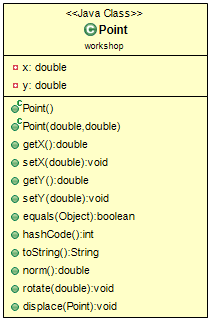
\includegraphics[width =0.4\textwidth]{Point.png}
	\caption{The (\texttt{Point()}) class}
	\label{point-class}
\end{figure}

Figure \ref{test-results-points} shows the test results for the \texttt{Point()} class tested by the unit tests implemented by my lab-partner.

\begin{figure}[!htb]
	\centering
	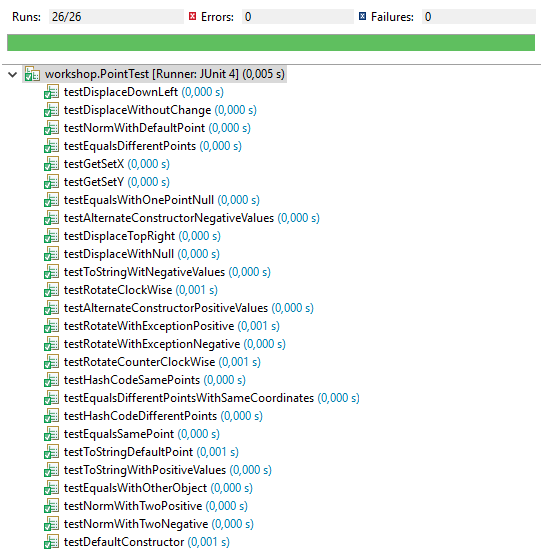
\includegraphics[width =0.9\textwidth]{pointTestResults.png}
	\caption{Test results (\texttt{Point()})}
	\label{test-results-points}
\end{figure}

%%%%%%%%%%%%%%%%%%%%%%%%%%%%%%%%%%%%%%%%%%%%%%%%%%%%%%%%%%%%%%%%%%%%%%%%%%%%%%%%%%%%%%%%%%%%%%%%%%%%%%%%%
%%%%%%%%%%%%%%%%%%%%%%%%%%%%%%%%%%%%%%%%%%%%%%%%%%%%%%%%%%%%%%%%%%%%%%%%%%%%%%%%%%%%%%%%%%%%%%%%%%%%%%%%%
%%%%%%%%%%%%%%%%%%%%%%%%%%%%%%%%%%%%%%%%%%%%%%%%%%%%%%%%%%%%%%%%%%%%%%%%%%%%%%%%%%%%%%%%%%%%%%%%%%%%%%%%%
\chapter{Test for the \texttt{Line()} class}
\label{exercise2}
For the second exercise the roles were switched. The team member who wrote the tests for the \texttt{Point()} class in the first exercise implemented the new class \texttt{Line()} and the team member who implemented the \texttt{Point()} class had to write the tests for the \texttt{Line()} class.\\
All Tests are listed in the appendix \ref{subsec: line-class-listing}. The following subsection will only show the tests for the given requirements and their corresponding methods.\\
\section {Constructor tests} 
The standard constructor for the \texttt{Line()} class should initialize a new \texttt{Line()} object without any points while an alternate constructor should receive an array of \texttt{Point}-objects to initialize the \texttt{Line} object's own \texttt{Point} array. The following tests evaluate these requirements:\\
\begin{lstlisting}
	@Test
	public void testDefaultConstructor() {
		Line line = new Line();
		assertTrue(line.length() == 0);
	}
	
	@Test
	public void testAlternateConstructor() {
		Point[] points = getPointsExampleData();
		Line line = new Line(points);
		assertEquals(3, line.length());
	}

	@Test
	public void testConstructorWithNull() {
		Line line = new Line(null);
		assertTrue(line.length() == 0);
	}
\end{lstlisting}
These tests cover the functionality of the constructors. The method \texttt{getPointsExampleData()} generates some \texttt{Point}-objects for the alternate constructor's test and will be shown in the appendix \ref{subsec: line-class-listing}.\\
The \texttt{length}-method is used here to evaluate the constructor's functionality. This might be a little controversial, because an unit test should only cover one method's functionality, but as long as the \texttt{Line} classes \texttt{Point} array is private or should at least it should be, there is no other way for observing a change in the array. Usually this isn't a problem, because the \texttt{length-method} has it's own test. As soon as there is a problem with the \texttt{length-method} the programmer will notice it.
\section {Tests for \texttt{length()} and \texttt{add()}} 
The \texttt{length()} method should return an integer value which represents the current size of the array inside the \texttt{Line} object receiving the method call. The \texttt{add()} method should make it possible to add a new \texttt{Point} object to the array. The following tests should cover their functionality:\\ 
\begin{lstlisting}
	@Test
	public void testAdd() {
		Line line = new Line();
		line.add(new Point());
		assertEquals(1, line.length());
	}
	
	@Test
	public void testAddWithNull() {
		Line line = new Line();
		line.add(null);
		assertEquals(0, line.length());
	}
	
	public void testLength() {
		Point[] points = getPointsExampleData();
		Line line = new Line(points);
		assertEquals(3, line.length());
	}
	
	public void testLengthAfterAdd() {
		Point[] points = getPointsExampleData();
		Line line = new Line(points);
		assertEquals(3, line.length());
		line.add(new Point(2.3543, 8.345));
		assertEquals(4, line.length());
	}
\end{lstlisting}
Once again the \texttt{length()} method is used to verify the \texttt{add()} method's correct functionality.
\section {Tests for \texttt{equals()}} 
The \texttt{equals()} method should compare two \texttt{Line} objects and determine if they share the same points. However the sequence of the points in the arrays inside the \texttt{Line} objects does not matter. The following tests evaluate this:\\ 
\begin{lstlisting}
	@Test
	public void testEqualsWithExactlySameLineObject() {
		Point[] points = getPointsExampleData();
		Line line = new Line(points);
		assertTrue(line.equals(line));
	}
	
	@Test
	public void testEqualsWithTwoLineObjectsWithSamePoints() {
		Point[] points = getPointsExampleData();
		Line line = new Line(points);
		Line line2 = new Line(points);
		assertTrue(line.equals(line2));
	}
	
	@Test
	public void testEqualsWithTwoLineObjectsWithSamePointsInDiffentOrder() {
		Point[] points = getPointsExampleData();
		Line line = new Line(points);
		Point[] points2 = new Point[3];
		points2[0] = new Point(2.4, -2.4);
		points2[2] = new Point(-0.2, 8.9);
		points2[1] = new Point(-4.4, -2.4);
		Line line2 = new Line(points2);
		assertTrue(line.equals(line2));
	}
	
	@Test
	public void testEqualsWithTwoLinesWithDifferentPoints() {
		Point[] points = getPointsExampleData();
		Line line = new Line(points);
		Point[] points2 = new Point[3];
		points2[0] = new Point(2.3, -1.4);
		points2[2] = new Point(-0.2, 2.9);
		points2[1] = new Point(-42.4, -2.4);
		Line line2 = new Line(points2);
		assertFalse(line.equals(line2));
	}
	
	@Test
	public void testEqualsWithFalseObject() {
		Point[] points = getPointsExampleData();
		Line line = new Line(points);
		// comparing a Line object to a Point object should return false...
		assertFalse(line.equals(new Point(3.9, 4.2)));
	}
	
	@Test
	public void testEqualsWithNull() {
		Point[] points = getPointsExampleData();
		Line line = new Line(points);
		assertFalse(line.equals(null));
	}
\end{lstlisting}
These tests cover the requirements while also ensuring the equals-method's stability. The method should be able to handle false objects as well as null-values.
\section {Tests for \texttt{hashCode()}} 
The \texttt{hashCode()}-method should generate the same hash-value for two \texttt{Line}-objects with the same \texttt{Point} array. The following tests verify the method's results:\\
\begin{lstlisting}
	@Test
	public void testHashCodeWithoutPoints() {
		Line line = new Line();
		Line line2 = new Line();
		assertEquals(line.hashCode(), line2.hashCode());
	}
	
	@Test
	public void testHashCodeWithSamePoints() {
		Line line = new Line(getPointsExampleData());
		Line line2 = new Line(getPointsExampleData());
		assertEquals(line.hashCode(), line2.hashCode());
	}
	
	@Test
	public void testHashCodeWithDifferentPoints() {
		Point[] points = getPointsExampleData();
		Line line = new Line(points);
		Line line2 = new Line();
		assertNotEquals(line.hashCode(), line2.hashCode());
	}
\end{lstlisting}
These tests should cover the \texttt{hashCode()}-method's functionality.
\section {Tests for \texttt{toString()}} 
The \texttt{Line} classes' \texttt{toString()}-method should be able to print the contained points in the console in the same way, the \texttt{Line} class does. the output should look like this:\\
\vspace{-10mm}
\begin{center}
	(( $\pm 0.0000E \pm 00$, $\pm 0.0000E \pm 00$ ),\\
	( $\pm 0.0000E \pm 00$, $\pm 0.0000E \pm 00$ ),\\
	...\\
	( $\pm 0.0000E \pm 00$, $\pm 0.0000E \pm 00$ )).
\end{center}
\vspace{-6mm}
The listing below shows the tests covering the method's behavior:\\
\begin{lstlisting}
	@Test
	public void testToString() {
		Point[] points = new Point[3];
		points[0] = new Point(0.00000021, 12345.1246);
		points[1] = new Point(-0.2556785, 1.1246365);
		points[2] = new Point(-235.25853467, -1.1246);
		Line line = new Line(points);
		String expectedOutout = "(( 2.4, -2.4 ),\n ( -0.2, 8.9 ),\n ( -4.4, -2.4 ))";
		assertEquals(expectedOutout, line.toString());
	}
\end{lstlisting}
There are not many problem that can occur here. So there are not too many tests for this method.
\section {Tests for \texttt{isValid()}} 
The \texttt{isValid()} should be able to check if the slope of the regression line and the intercept with the Y-axis can be calculated. There are a few cases when this should not be possible. When the number of points in the line is either 0 or 1, the slope cannot be determined. The same happens when all points have the same coordinates or have the same x-coordinate. So here are some test which verify that the \texttt{isValid()} method can handle these cases correctly:\\
\begin{lstlisting}
	@Test
	public void testIsValidWithZeroPoints() {
		Line line = new Line();
		assertFalse(line.isValid());
	}
	
	@Test
	public void testIsValidWithOnePoint() {
		Line line = new Line();
		line.add(new Point(2.1, 4.3));
		assertFalse(line.isValid());
	}
	
	@Test
	public void testIsValidWithManyPoints() throws RegressionFailedException {
		Point[] points = getPointsExampleData();
		Line line = new Line(points);
		assertTrue(line.isValid());
	}
	
	@Test
	public void testIsValidWithTwoPointsWithSameCoordinates() {
		Point[] points = new Point[2];
		points[0] = new Point(2.1, 2.1);
		points[1] = new Point(2.1, 2.1);
		Line line = new Line(points);
		assertFalse(line.isValid());
	}
	
	@Test
	public void testIsValidWithTwoPointsWithSameXCoordinates() {
		Point[] points = new Point[2];
		points[0] = new Point(2.1, 23.34);
		points[1] = new Point(2.1, 21.23);
		Line line = new Line(points);
		assertFalse(line.isValid());
	}
\end{lstlisting}
These tests do not evaluate the output for slope and intercept, as there are different methods for that.
\section {Tests for \texttt{slope()}} 
The \texttt{slope()} method should be able to calculate the linear regression line for the points contained inside the \texttt{Line} object. If the slope cannot be calculated a new \texttt{RegressionFailedException} must be thrown. The following tests check the functionality for this method:\\
\begin{lstlisting}
	@Test
	public void testSlopeWithTwoValidPoints() throws RegressionFailedException{
		// very simple tests
		Point[] points = new Point[2];
		points[0] = new Point(0, 0);
		points[1] = new Point(1, 1);
		Line line = new Line(points);
		double slope = line.slope();
		assertEquals(1, slope, 0);
	}
	
	@Test
	public void testSlopeWithValidPoints() throws RegressionFailedException{
		// more complex parameters
		Point[] points = new Point[6];
		points[0] = new Point(0.2, 0);
		points[1] = new Point(1, 3.12);
		points[2] = new Point(3.23, 1);
		points[3] = new Point(-1.5, 1.3);
		points[4] = new Point(4.9, 12.2);
		points[5] = new Point(3.32, 2);
		Line line = new Line(points);
		double slope = line.slope();
		assertEquals(1.2, slope, 0.03);
	}
	
	@Test(expected = RegressionFailedException.class)
	public void testSlopeWithSamePoints() throws RegressionFailedException{
		Point[] points = new Point[2];
		points[0] = new Point(0, 0);
		points[1] = new Point(0, 0);
		// these points have the same coordinates. 
		// So the slope can't be calculated with these two.
		Line line = new Line(points);
		line.slope();
	}
\end{lstlisting}
The first test works with very simple points evaluating the very functionality of the \texttt{slope} method by using Points that generate a regression line with the value '1' as slope. The second test uses some more complex point and check the result. The third test uses one of the cases discussed in the \texttt{isValid()} section to force the occurrence of a \texttt{RegressionFailedException}.
\section{Tests for \texttt{intercept()}}
the method \texttt{intercept()} should determine the interception of the regression line with the Y-axis. There are some cases, where this cannot be done. Then a new \texttt{RegressionFailedException} should be thrown. When the all the points in the line have the same x-coordinate, the slope is infinite and there can never be an interception with the y-axis. The following tests evaluate the behavior of the method \texttt{intercept()}:\\
\begin{lstlisting}
	@Test
	public void testInterceptIWithValidPoints() throws RegressionFailedException{
		Point[] points = new Point[2];
		points[0] = new Point(0, 0);
		points[1] = new Point(1, 1);
		Line line = new Line(points);
		double intercept = line.intercept();
		assertEquals(0, intercept, 0);
	}
	
	@Test(expected = RegressionFailedException.class)
	public void testInterceptIWithInvalidPoints() throws RegressionFailedException{
		Point[] points = new Point[2];
		points[0] = new Point(0, 0);
		points[1] = new Point(0, 1);
		// with these points the line lies on the y-axis. therefore slope can't be calculated. 
		// And without slope, there is no intercept.
		Line line = new Line(points);
		line.intercept();
	}
\end{lstlisting}
Again there is one test for the normal behavior of the \texttt{intercept()} method and another test for one of the cases discussed above where intercept cannot be determined and a \texttt{RegressionFailedException} is expected.\\
In the following (Figure \ref{test-results-line}) the results of the tests created for the line class are shown.
\begin{figure}[!htb]
	\centering
	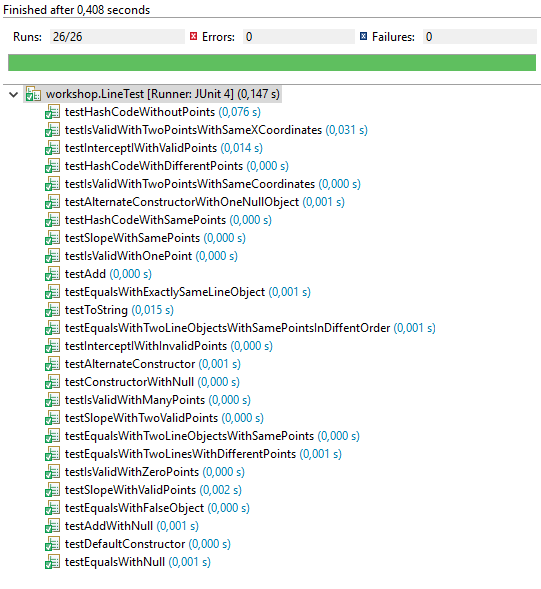
\includegraphics[width =0.9\textwidth]{lineTestResults.png}
	\caption{Test results (\texttt{Line()})}
	\label{test-results-line}
\end{figure}

Finally figure \ref{line-uml} shows the UML diagram of the \texttt{Line()} class.
\begin{figure}[!htb]
	\centering
	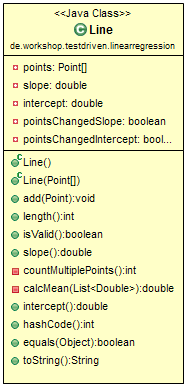
\includegraphics[width =0.3\textwidth]{LineUML.png}
	\caption{UML diagram of the \texttt{Line()} class}
	\label{line-uml}
\end{figure}

%%%%%%%%%%%%%%%%%%%%%%%%%%%%%%%%%%%%%%%%%%%%%%%%%%%%%%%%%%%%%%%%%%%%%%%%%%%%%%%%%%%%%%%%%%%%%%%%%%%%%%%%%
%%%%%%%%%%%%%%%%%%%%%%%%%%%%%%%%%%%%%%%%%%%%%%%%%%%%%%%%%%%%%%%%%%%%%%%%%%%%%%%%%%%%%%%%%%%%%%%%%%%%%%%%%
%%%%%%%%%%%%%%%%%%%%%%%%%%%%%%%%%%%%%%%%%%%%%%%%%%%%%%%%%%%%%%%%%%%%%%%%%%%%%%%%%%%%%%%%%%%%%%%%%%%%%%%%%
\chapter{The \texttt{LinearRegression} Application}
\label{exercise3}
The third exercise should be solved individually by each student. There were two files with example data provided (data\_short.dat and data\_long.dat) as well as a java library 'readFile.jar' containing classes that could read the data inside these two files. An example code on how to use the library was provided too.\\
The two .dat files contained multiple sequences of double-pairs which could be parsed into \texttt{Point} and \texttt{Line} Objects. This was the subject of this exercise. Both files should be parsed by the program and the results should be analyzed to get the following statistics for the given data:
\begin{itemize}
	\item The total number of lines, valid and invalid counted separately.
	\item The average number of points per valid lines.
	\item The average slope and its standard deviation for all valid lines.
	\item The average y-intercept and its standard deviation for all valid lines.
\end{itemize}
Figure \ref{results-short} shows the results for the lines from file data\_short.dat
\begin{figure}[!htb]
	\centering
	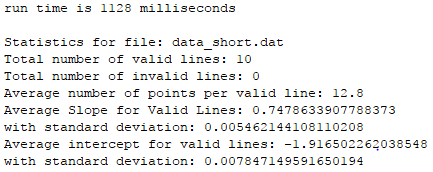
\includegraphics[width =0.7\textwidth]{outputShort_new.png}
	\caption{Results from data\_short.dat}
	\label{results-short}
\end{figure}
and figure \ref{results-long} the results from data\_long.dat.
\begin{figure}[!htb]
 	\centering
 	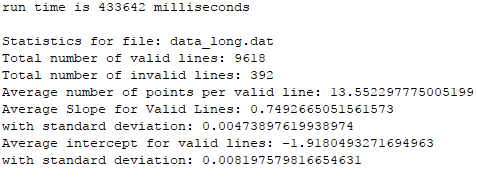
\includegraphics[width =0.7\textwidth]{outputLong_new.png}
 	\caption{Results from data\_long.dat}
 	\label{results-long}
\end{figure}
\newpage
The code for the \texttt{LinearRegression} Application will be shown in the appendix \ref{subsec: analyser-class-listing}. The classes' name is \texttt{LinearRegressionProgram}. Figure \ref{uml-exercise3} shows the UML diagram for the complete program and figure \ref{sequ} shows the sequence diagram for the application.
\begin{figure}[!htb]
	\centering
	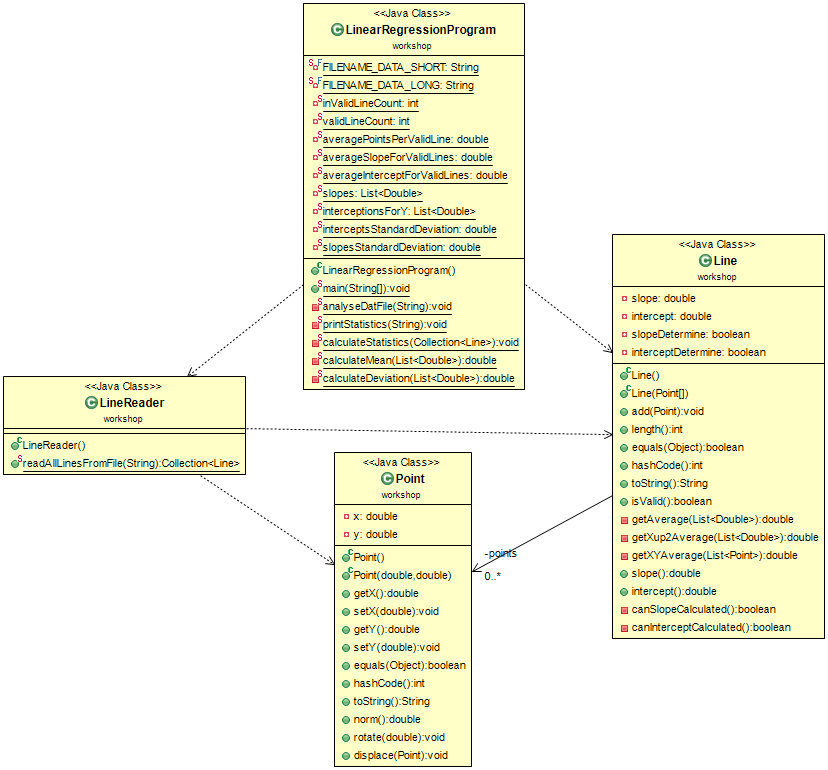
\includegraphics[width =1.0\textwidth]{LinearRegressionUML.PNG}
	\caption{UML class diagram for the \texttt{LinearRegression} application}
	\label{uml-exercise3}
\end{figure}

\begin{figure}[!htb]
	\centering
	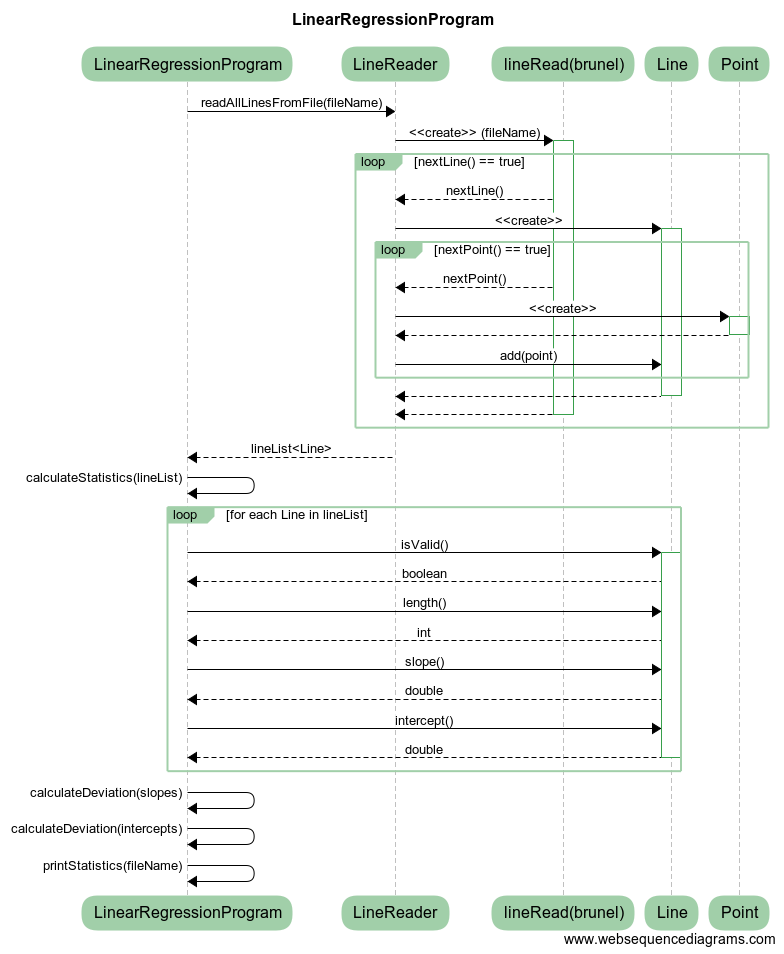
\includegraphics[width =0.85\textwidth]{LinearRegressionProgram.png}
	\caption{Sequence diagram for the \texttt{LinearRegression} application}
	\label{sequ}
\end{figure}

%%%%%%%%%%%%%%%%%%%%%%%%%%%%%%%%%%%%%%%%%%%%%%%%%%%%%%%%%%%%%%%%%%%%%%%%%%%%%%%%%%%%%%%%%%%%%%%%%%%%%%%%%
%%%%%%%%%%%%%%%%%%%%%%%%%%%%%%%%%%%%%%%%%%%%%%%%%%%%%%%%%%%%%%%%%%%%%%%%%%%%%%%%%%%%%%%%%%%%%%%%%%%%%%%%%
%%%%%%%%%%%%%%%%%%%%%%%%%%%%%%%%%%%%%%%%%%%%%%%%%%%%%%%%%%%%%%%%%%%%%%%%%%%%%%%%%%%%%%%%%%%%%%%%%%%%%%%%%
\chapter{Evaluating the performance}
\label{exercise4}
In last exercise of this workshop the time the program needed to read in the data and the time to perform the required operations with the number of points in the data sets should be evaluated.\\
To do this, the provided example code for time calculations were used to get the following data for the file data\_short.dat:\\

\begin{figure}[!htb]
	\centering
	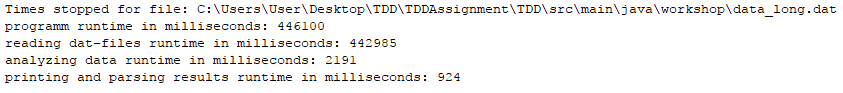
\includegraphics[width =1.0\textwidth]{timedata.png}
	\caption{Stopped durations for the different operation in the \texttt{LinearRegression} application in milliseconds}
	\label{timelong}
\end{figure}

This shows that the time the program needs to read the data from data\_short.dat is a lot longer than the duration stopped for the analyzing process. Therefore the reading time and how it depends on the number of points in the lines were further investigated by using the following HashMap in the \texttt{LineReader} class:\\
\begin{lstlisting}
	private static Map<Integer, List<Long>> timeData = new HashMap<Integer, List<Long>>();
\end{lstlisting}
At the start of each run through the loop reading a line from the dat file, a timestamp was initialized. The same was done at the end of each run through the loop. After that the duration between those timestamps was calculated and saved into the HashMap using this code:\\
\begin{lstlisting}
	// Get the duration it took, to read a single line in milliseconds.
	long timeToReadLine = endLineTimeStamp.getTime() - startLineTimeStamp.getTime();
	if (timeData.containsKey(line.length())) {
		timeData.get(line.length()).add(timeToReadLine);
	} else {
		List<Long> timeList = new ArrayList<>();
		timeList.add(timeToReadLine);
		timeData.put(line.length(), timeList);
	}
}
\end{lstlisting}
The number of points is used as key while the duration is added to the associated list of durations. Using this resulted in a lot of time data for each line length, which had to be normalized in the main application using the following method:\\
\begin{lstlisting}
	// Gets the avarage for the time it took to process a line with a certain 
	// amount of points from raw timestamp-data
	private static Map<Integer, Long> normalizeTimeData(Map<Integer, List<Long>> data){
		Map<Integer, Long> normalizedData = new HashMap<Integer, Long>();
		for (Integer key : data.keySet()){
			List<Long> stoppedTimes = data.get(key);
			long avarage = 0;
			long sum = 0;
			for (Long time : stoppedTimes){
				sum += time;
			}
			if(stoppedTimes.size() != 0){
				avarage = (long) sum / stoppedTimes.size();
			}
			normalizedData.put(key, avarage);
		}
		return normalizedData;
	}
\end{lstlisting}
This method's result is parsed into an Excel file in the project path. the data from the Excel file is shown in the table \ref{table}. The class responsible for writing the Excel File is listed in the appendix \ref{subsec: ExcelWriter-listing}.

\begin{table}[!htb]
	\centering
	\begin{tabular}{|c|c|}
		\hline
		Number of Points & Time to read (ms) \\ \hline
		1                & 2                 \\ \hline
		2                & 5                 \\ \hline
		3                & 7                 \\ \hline
		4                & 10                \\ \hline
		5                & 12                \\ \hline
		6                & 15                \\ \hline
		7                & 18                \\ \hline
		8                & 20                \\ \hline
		9                & 23                \\ \hline
		10               & 34                \\ \hline
		11               & 38                \\ \hline
		12               & 42                \\ \hline
		13               & 45                \\ \hline
		14               & 49                \\ \hline
		15               & 52                \\ \hline
		16               & 56                \\ \hline
		17               & 60                \\ \hline
		18               & 63                \\ \hline
		19               & 66                \\ \hline
		20               & 70                \\ \hline
		21               & 73                \\ \hline
		22               & 77                \\ \hline
		23               & 80                \\ \hline
		24               & 84                \\ \hline
		25               & 87                \\ \hline
	\end{tabular}
	\vspace{3mm}
	\caption{Number of points and their times}
	\label{table}
\end{table}

Additionally, Figure \ref{plot} shows the plot of time needed to read and create a line over the number of point in this line from the Excel file. It can be seen that the time increases fairly linear with number of point. But there also is a leap from nine points to ten. This must be caused by the class \texttt{lineRead} which was provided to reading in the data.
\begin{figure}[!htb]
	\centering
	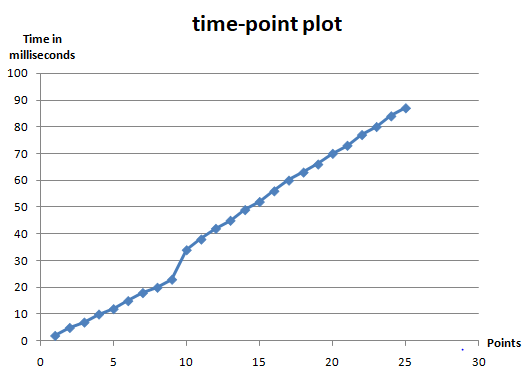
\includegraphics[width =0.75\textwidth]{timepointplot.png}
	\caption{Time-Point plot}
	\label{plot}
\end{figure}
